\documentclass[12pt]{article}

% ---------- Packages ----------
\usepackage[margin=1in]{geometry}
\usepackage{graphicx}
\usepackage{booktabs}
\usepackage{amsmath}
\usepackage{hyperref}
\usepackage{natbib}
\usepackage{microtype}
\usepackage{setspace}
\usepackage{caption}
\usepackage{float}
\usepackage[T1]{fontenc}
\usepackage[utf8]{inputenc}
\usepackage{lmodern}
\usepackage{xcolor}

\hypersetup{
    colorlinks=true,
    linkcolor=blue,
    citecolor=blue,
    urlcolor=blue
}

\doublespacing

% ---------- Title ----------
\title{%
  \textbf{Forecasting Antimicrobial Resistance Trends Using Machine Learning \\
  on WHO GLASS Surveillance Data: A Retrieval-Augmented Generation \\
  Approach for Policy Decision Support}
}

\author{
  Md Tanvir Hasan Turja \\
  MSc Data Science, Middlesex University London \\
  London, United Kingdom \\
  \url{https://github.com/TanvirTurja}
}

\date{February 2026}

% ---------- Document ----------
\begin{document}

\maketitle

% ---------- Abstract ----------
\begin{abstract}
Antimicrobial resistance (AMR) is a growing global crisis projected to cause 10 million deaths per year by 2050. While the WHO Global Antimicrobial Resistance and Use Surveillance System (GLASS) provides standardized surveillance data across 44 countries, few studies have applied machine learning to forecast population-level resistance trends from this data. This paper presents a two-component framework for AMR trend forecasting and evidence-grounded policy decision support. We benchmark six models---Naive, Linear Regression, Ridge Regression, XGBoost, LightGBM, and LSTM---on 5,909 WHO GLASS observations across six WHO regions (2021--2023). XGBoost achieved the best performance with a test MAE of 7.07\% and R\textsuperscript{2} of 0.854, outperforming the naive baseline by 83.1\%. Feature importance analysis identified the prior-year resistance rate as the dominant predictor (50.5\% importance), while regional MAE ranged from 4.16\% (European Region) to 10.14\% (South-East Asia Region), reflecting disparities in GLASS data quality. We additionally implemented a Retrieval-Augmented Generation (RAG) pipeline combining a ChromaDB vector store of WHO policy document excerpts with a locally deployed Phi-3 Mini language model, injecting forecast context into each query to produce source-attributed, hallucination-constrained policy answers. Together, these components demonstrate the feasibility of integrating AMR surveillance forecasting with intelligent policy question answering using openly available data and locally deployable models.

\noindent\textbf{Keywords:} antimicrobial resistance, WHO GLASS, machine learning, XGBoost, LSTM, time series forecasting, retrieval-augmented generation, public health surveillance, policy decision support
\end{abstract}

% ---------- 1. Introduction ----------
\section{Introduction}

Antimicrobial resistance (AMR) represents one of the most urgent threats to global health in the twenty-first century. In 2019, AMR was directly responsible for an estimated 1.27 million deaths worldwide and was associated with an additional 4.95 million deaths, with the highest burden concentrated in Sub-Saharan Africa and South Asia \citep{murray2022}. Without coordinated international action, AMR is projected to cause 10 million deaths per year by 2050, surpassing cancer as the leading cause of death globally \citep{oneill2016, dekraker2016}. These projections carry wide-ranging consequences across patient outcomes, healthcare systems, and national economies \citep{dadgostar2019, tang2023}, and have prompted global political responses including the WHO Global Action Plan on Antimicrobial Resistance \citep{who2015gap, sugden2016}.

A critical prerequisite for effective AMR governance is the ability to monitor and forecast resistance trends across pathogens, antibiotics, and geographic regions. The WHO Global Antimicrobial Resistance and Use Surveillance System (GLASS) was established to provide standardized, comparable AMR data from national surveillance networks worldwide \citep{who2022glass, who2023manual}. GLASS data captures resistance rates across multiple pathogen-antibiotic combinations and has been used to demonstrate the relationship between antibiotic consumption and resistance across participating countries \citep{ajulo2024}. However, GLASS data availability remains uneven across regions, with participation concentrated in higher-income countries and more established surveillance systems.

Machine learning has attracted growing interest as a tool for AMR prediction, primarily applied to clinical isolate datasets to classify susceptibility or resistance at the level of individual bacterial samples \citep{sakagianni2023, kim2022}. These approaches have shown promise within clinical laboratory settings but do not directly address population-level forecasting of resistance trends from surveillance data. The temporal and geographic structure of GLASS data, covering resistance rates over time and across countries, calls for time series forecasting approaches rather than isolate-level classification.

Beyond forecasting, there is a parallel need for tools that make AMR surveillance findings interpretable and actionable for policymakers and public health practitioners. Large language models (LLMs) and Retrieval-Augmented Generation (RAG) systems \citep{lewis2020} offer a promising direction for this purpose, enabling natural-language policy queries to be answered with evidence grounded in specific source documents rather than model parameters alone.

This paper addresses both gaps with a two-component framework. First, we benchmark six machine learning models on WHO GLASS surveillance data (2021--2023) across 44 countries to forecast resistance rates at the country-pathogen-antibiotic level. Second, we implement a RAG pipeline that combines forecast results with retrieved WHO policy documents to answer natural-language questions about AMR policy and resistance trends.

Our main contributions are:
\begin{enumerate}
    \item A multi-model benchmark (Naive, Linear Regression, Ridge Regression, XGBoost, LightGBM, LSTM) on WHO GLASS surveillance data for population-level resistance rate forecasting, identifying XGBoost as the best-performing approach with a test MAE of 7.07\% and R\textsuperscript{2} of 0.854.
    \item A feature importance and regional error analysis identifying the resistance lag feature as the dominant predictor and highlighting geographic disparities in forecast accuracy tied to GLASS participation rates.
    \item A locally deployed RAG system grounding AMR policy answers in retrieved WHO document chunks and forecast context, without requiring proprietary cloud APIs.
\end{enumerate}

% ---------- 2. Related Work ----------
\section{Related Work}

\subsection{Machine Learning for AMR Prediction}

The application of machine learning to AMR has grown substantially over the past decade. \citet{sakagianni2023} provided a comprehensive literature review of ML approaches to AMR prediction, covering random forests, support vector machines, neural networks, and gradient boosting methods. \citet{kim2022} reviewed current practice and limitations from a clinical perspective, noting that most existing work focuses on isolate-level susceptibility classification rather than population-level temporal forecasting. Both reviews identified a gap in approaches using surveillance data for anticipatory forecasting of resistance trends, which is the primary focus of this work.

\subsection{Gradient Boosting for Epidemiological Forecasting}

Gradient boosting methods have demonstrated consistent advantages over classical statistical models for infectious disease time series. \citet{alim2020} compared XGBoost and ARIMA for predicting human brucellosis incidence in China, finding that XGBoost achieved a test MAPE of 7.64\% compared to 17.68\% for ARIMA, attributing XGBoost's advantage to its ability to model nonlinear patterns without stationarity assumptions. \citet{fang2022} replicated this finding for COVID-19 transmission forecasting in the United States. \citet{ahn2023} demonstrated that ensemble gradient boosting (XGBoost, LightGBM, CatBoost) combined with attention-based CNN-LSTM achieved strong performance for environmental time series forecasting, validating both XGBoost \citep{chen2016} and LightGBM \citep{ke2017} in a forecasting context with temporal structure similar to our AMR dataset.

\subsection{LSTM Networks for Epidemic Forecasting}

\citet{chimmula2020} applied LSTM to model COVID-19 transmission dynamics in Canada, demonstrating the feasibility of LSTM for short-horizon epidemic forecasting and motivating its inclusion in our model comparison. In our evaluation, LSTM achieves performance comparable to gradient boosting (MAE: 7.16\%), confirming that the limited temporal dataset is the constraining factor rather than model architecture choice.

\subsection{Retrieval-Augmented Generation}

\citet{lewis2020} introduced the RAG framework, combining a dense retrieval component with a sequence-to-sequence language model to answer knowledge-intensive questions by grounding responses in retrieved document passages. Our work applies RAG to the AMR domain, integrating WHO policy documents with ML-derived forecast context to support evidence-based policy queries. To our knowledge, this is the first application of RAG specifically for AMR policy question answering informed by GLASS surveillance forecasts.

% ---------- 3. Data and Methods ----------
\section{Data and Methods}

\subsection{Dataset}

We used the WHO Global Antimicrobial Resistance and Use Surveillance System (GLASS) dataset covering the years 2021--2023 \citep{who2022glass, who2023manual}. The dataset contains standardized resistance observations collected from national surveillance networks across 44 countries spanning six WHO geographic regions. The final processed dataset comprised 5,909 observations after cleaning. Each observation records a unique combination of country, pathogen, antibiotic, and year. The target variable is the resistance percentage, defined as the proportion of tested isolates that demonstrated resistance to the corresponding antibiotic (Table~\ref{tab:dataset}).

\begin{table}[H]
\centering
\caption{Dataset characteristics.}
\label{tab:dataset}
\begin{tabular}{ll}
\toprule
\textbf{Attribute} & \textbf{Value} \\
\midrule
Years covered & 2021--2023 \\
Number of countries & 44 \\
WHO regions & 6 \\
Total observations & 5,909 \\
Target variable & Resistance percentage (\%) \\
Income groups & High, Upper-middle, Lower-middle, Low, Unknown \\
\bottomrule
\end{tabular}
\end{table}

The AMR-consumption relationship documented by \citet{ajulo2024} across GLASS-participating countries informed our feature selection, particularly the inclusion of antibiotic consumption as a predictive feature.

\subsection{Features}

Input features for all supervised models included: pathogen name, antibiotic name, country or territory, WHO region, income group (World Bank classification), year, resistance lag (resistance percentage in the prior year for the same pathogen-antibiotic-country combination), and antibiotic consumption (defined daily doses per 1,000 inhabitants per day). High-cardinality categorical features were encoded using target encoding applied within the training set to prevent data leakage.

\subsection{Preprocessing}

Missing values in the target variable and lag features were imputed using the median resistance rate for the corresponding pathogen-antibiotic pair. The dataset was split temporally: 2021--2022 observations for training, 2022 observations for validation, and 2023 observations for the held-out test set, preventing information leakage from future time points into training.

\subsection{Models}

We compared six models of increasing complexity:

\textbf{Naive Baseline.} Predicts each observation's resistance rate as equal to the prior year's resistance rate (lag1). This represents the minimum performance threshold any model must surpass.

\textbf{Linear Regression.} Ordinary least squares regression on all encoded features.

\textbf{Ridge Regression.} L2-regularized linear regression; regularization parameter selected via cross-validation.

\textbf{XGBoost.} Scalable gradient boosting framework using decision trees as base learners \citep{chen2016}. XGBoost has consistently outperformed classical statistical models for infectious disease time series forecasting \citep{alim2020, fang2022}.

\textbf{LightGBM.} Histogram-based gradient boosting algorithm offering efficient training on tabular data \citep{ke2017}. Gradient boosting ensembles including LightGBM have demonstrated strong performance on biological time series \citep{ahn2023}.

\textbf{LSTM.} Single-layer Long Short-Term Memory network with sequences of length 1 given the limited temporal span of the dataset \citep{chimmula2020}. Trained on CPU due to GPU driver incompatibility with the available PyTorch build.

Hyperparameters for XGBoost and LightGBM were tuned via grid search over learning rate, maximum depth, number of estimators, and subsampling ratio. LSTM training used the Adam optimizer ($\text{lr}=0.001$) with early stopping on validation MAE.

\subsection{Evaluation Metrics}

All models were evaluated on the held-out 2023 test set using Mean Absolute Error (MAE), Root Mean Square Error (RMSE), and R\textsuperscript{2}. Regional MAE was additionally computed by disaggregating test predictions by WHO region.

\subsection{RAG Pipeline}

To augment model forecasts with interpretable policy context, we implemented a Retrieval-Augmented Generation (RAG) system \citep{lewis2020}.

\textbf{Knowledge base.} Six curated WHO policy document excerpts covering: carbapenem resistance and ESKAPE pathogens, the Global Action Plan on AMR \citep{who2015gap}, the AWaRe antibiotic classification, AMR surveillance investment priorities for LMICs, and regional resistance trends from GLASS data.

\textbf{Embedding and retrieval.} Document chunks were encoded using the \texttt{all-MiniLM-L6-v2} sentence transformer model and stored in a ChromaDB vector database. The top 3 most semantically relevant chunks were retrieved per query using cosine similarity.

\textbf{Language model.} Retrieved chunks were combined with XGBoost forecast findings and regional MAE results to construct a structured prompt submitted to Phi-3 Mini (3.8B parameters) via Ollama. The system prompt explicitly prohibited fabricated citations, restricting source references to retrieved document chunk labels only.

\textbf{Forecast context injection.} Each query received an appended context block summarizing XGBoost feature importances, regional MAE values, and the model performance comparison table.

% ---------- 4. Results ----------
\section{Results}

\subsection{Model Performance Comparison}

Table~\ref{tab:results} presents the performance of all six models on the 2023 held-out test set.

\begin{table}[H]
\centering
\caption{Model performance on the 2023 held-out test set.}
\label{tab:results}
\begin{tabular}{lcccc}
\toprule
\textbf{Model} & \textbf{Test MAE (\%)} & \textbf{Test RMSE (\%)} & \textbf{Test R\textsuperscript{2}} & \textbf{vs. Naive} \\
\midrule
Naive Baseline       & 41.83 & 48.15 & ---   & Reference \\
Linear Regression    & 8.23  & 11.96 & 0.821 & 80.3\% \\
Ridge Regression     & 8.25  & 11.95 & 0.821 & 80.3\% \\
LightGBM             & 7.17  & 10.84 & 0.853 & 82.9\% \\
LSTM                 & 7.16  & 10.10 & 0.872 & 82.9\% \\
\textbf{XGBoost}     & \textbf{7.07} & \textbf{10.80} & \textbf{0.854} & \textbf{83.1\%} \\
\bottomrule
\end{tabular}
\end{table}

\begin{figure}[H]
\centering
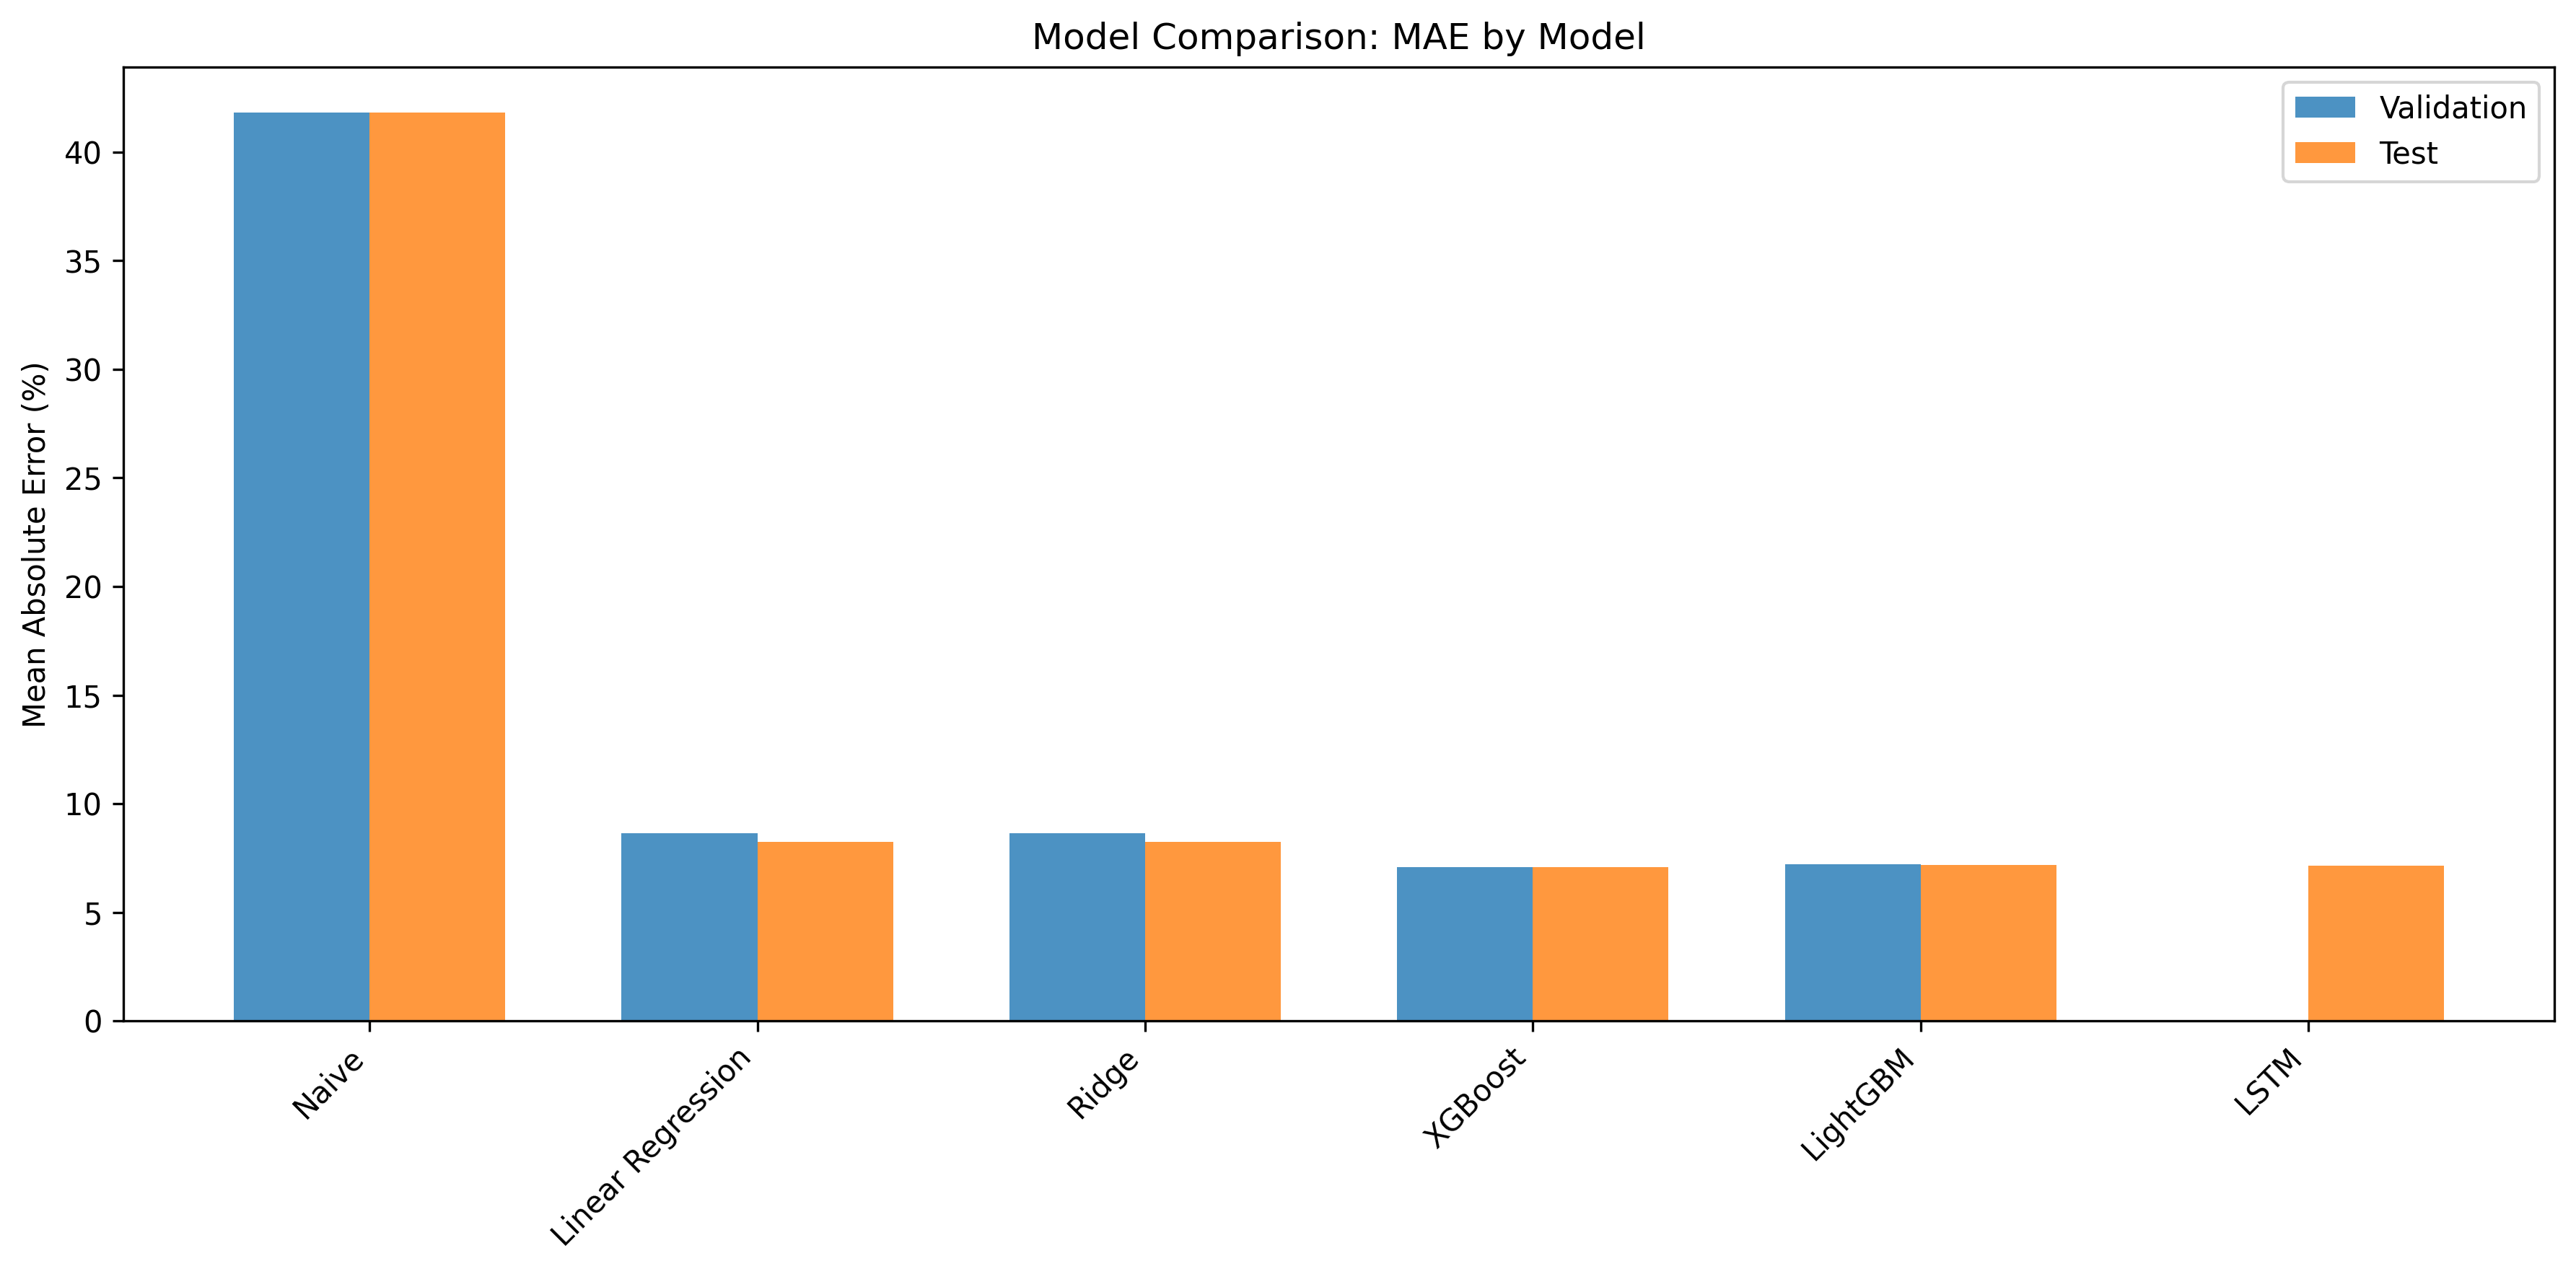
\includegraphics[width=0.85\textwidth]{model_comparison.png}
\caption{Model performance comparison across all six models on validation and test sets. XGBoost achieves the lowest test MAE (7.07\%), with LightGBM and LSTM closely behind.}
\label{fig:model_comparison}
\end{figure}

XGBoost achieved the lowest test MAE of 7.07\% and R\textsuperscript{2} of 0.854, outperforming the naive baseline by 83.1\%. This is consistent with prior findings demonstrating XGBoost superiority over statistical baselines for infectious disease time series \citep{alim2020, fang2022}. Gradient boosting models and the LSTM achieved comparable performance with a spread of less than 0.15 percentage points in MAE. The convergence of deep learning and tree-based performance is expected given the limited three-year temporal span; LSTM networks typically provide greater advantage over longer sequences \citep{chimmula2020}.

\subsection{Feature Importance Analysis}

Table~\ref{tab:importance} shows the top five XGBoost features by gain-based importance.

\begin{table}[H]
\centering
\caption{XGBoost feature importances (gain-based, top 5).}
\label{tab:importance}
\begin{tabular}{clc}
\toprule
\textbf{Rank} & \textbf{Feature} & \textbf{Importance (\%)} \\
\midrule
1 & Resistance\_lag1 (prior year resistance) & 50.5 \\
2 & CountryTerritoryArea                    & 9.0  \\
3 & AntibioticName                          & 6.7  \\
4 & PathogenName                            & 6.0  \\
5 & Antibiotic consumption (DID)            & 4.8  \\
\bottomrule
\end{tabular}
\end{table}

\begin{figure}[H]
\centering
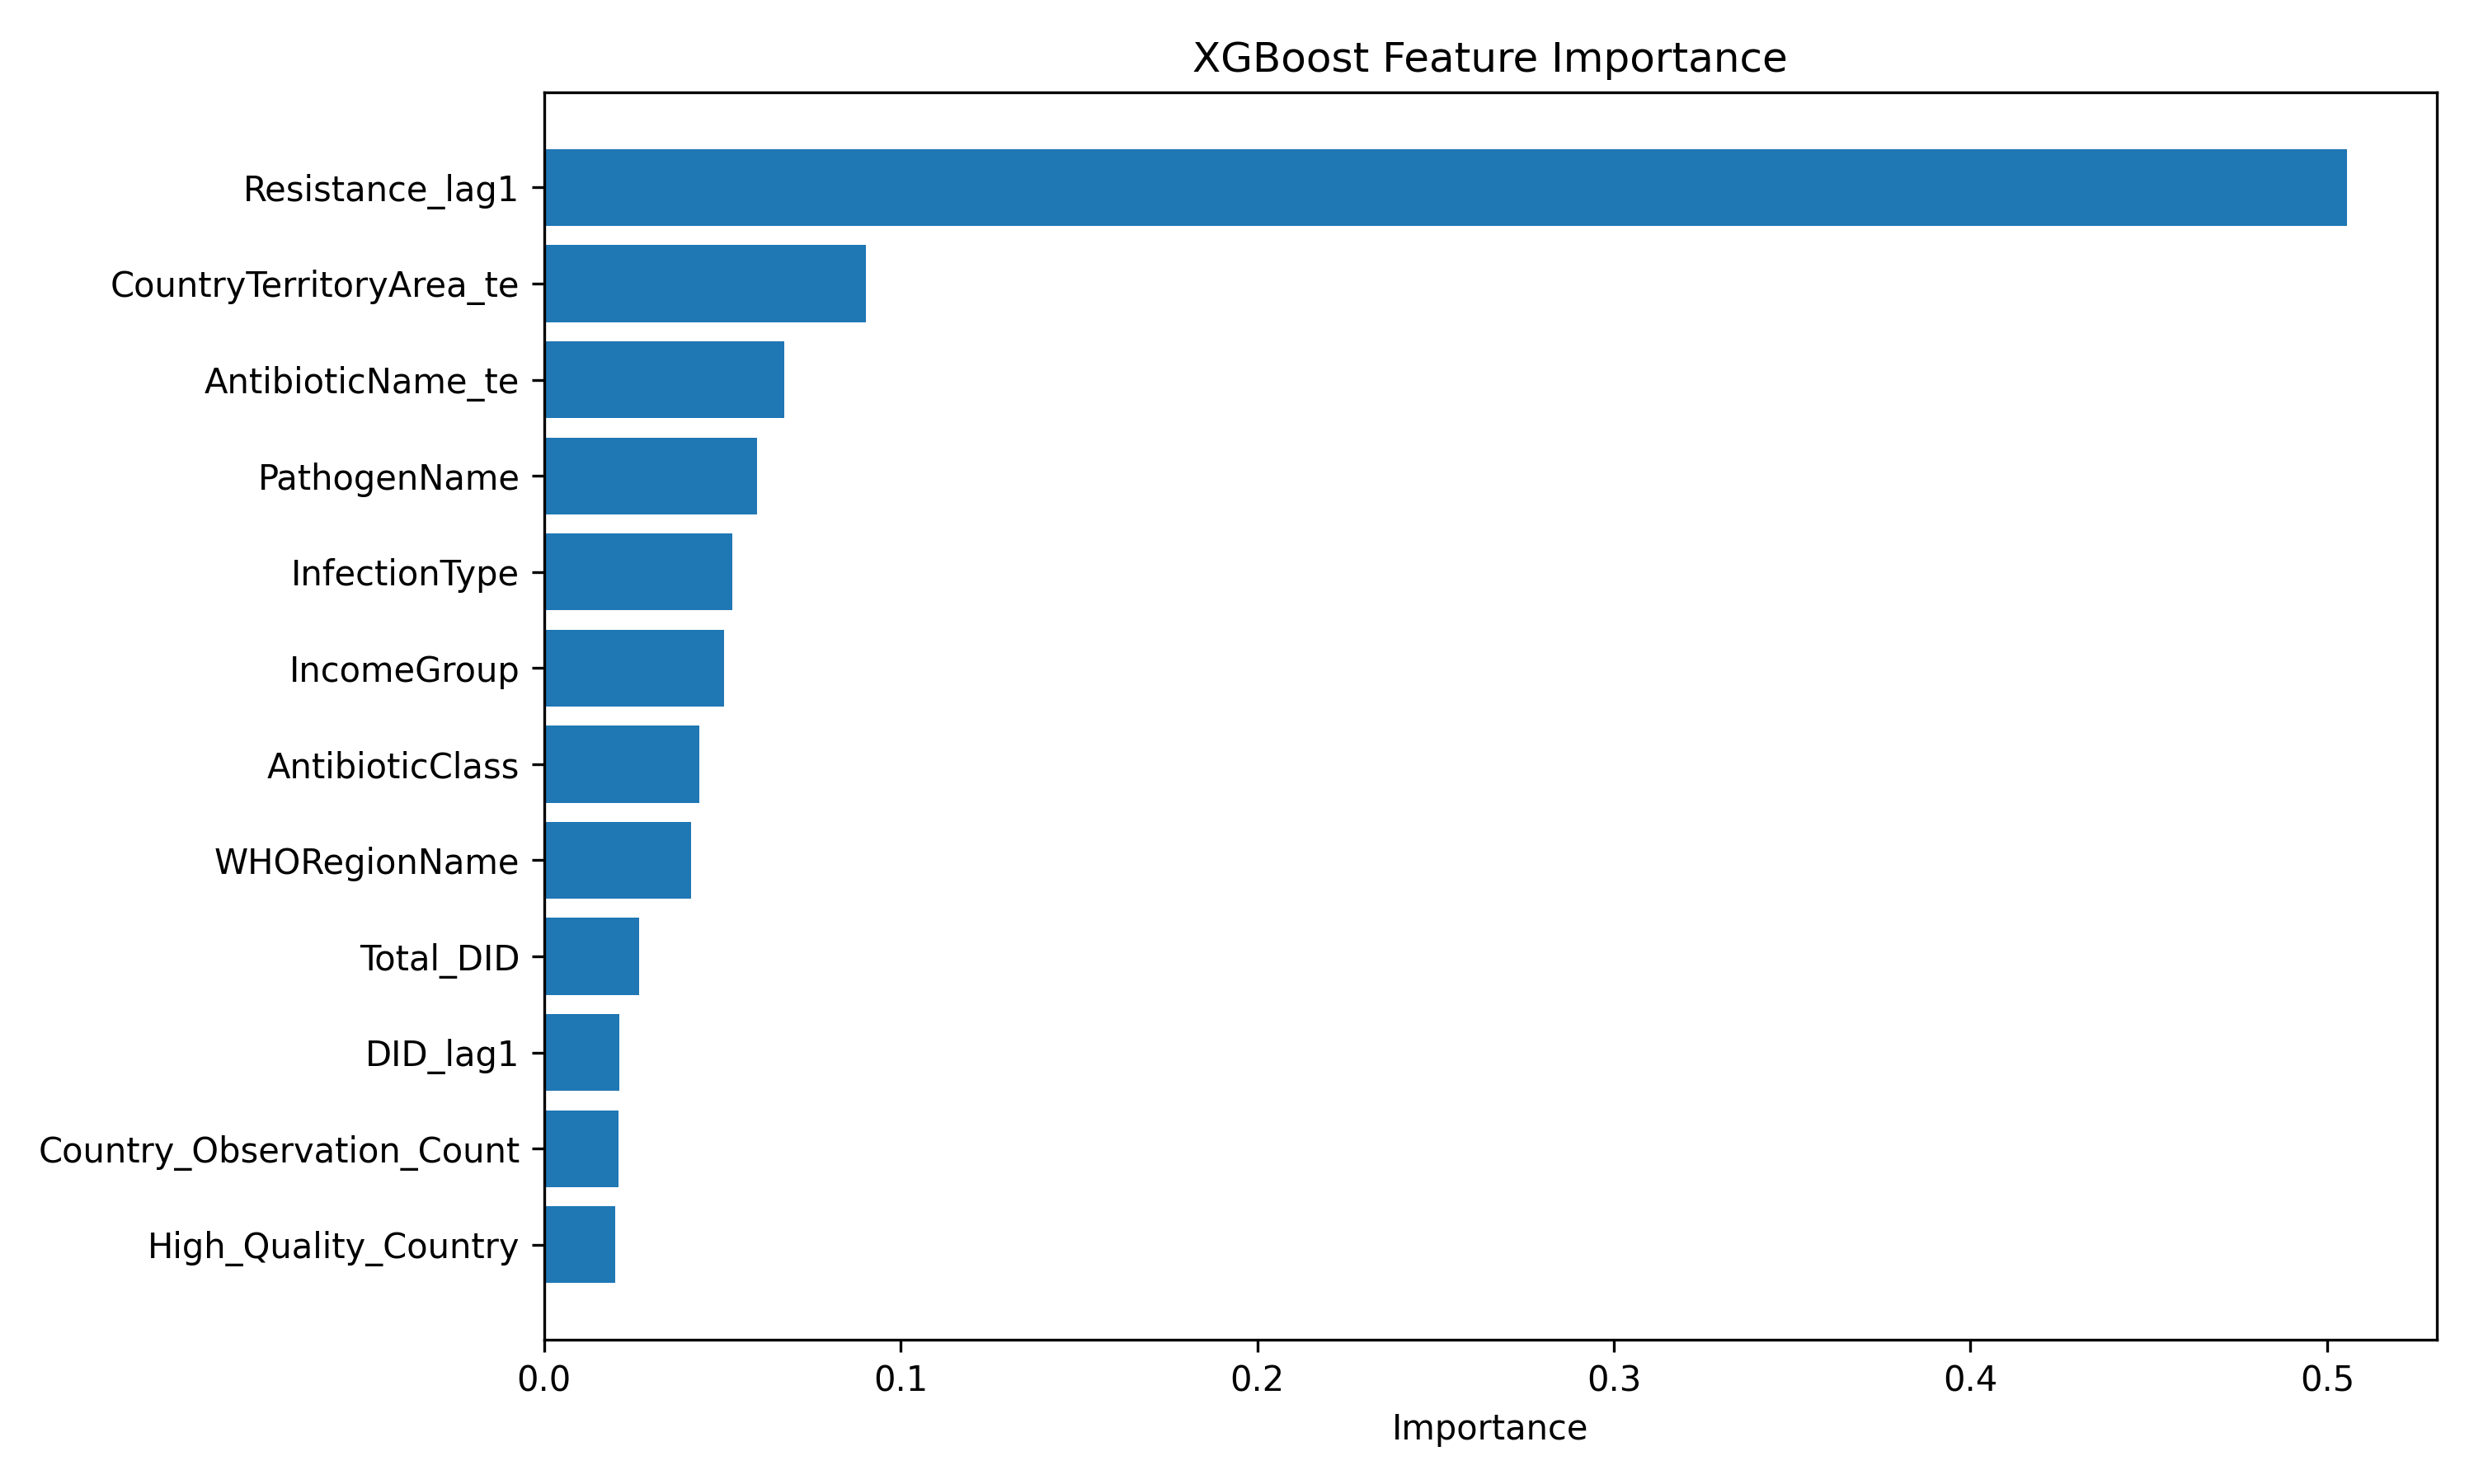
\includegraphics[width=0.85\textwidth]{xgb_feature_importance.png}
\caption{XGBoost feature importance (gain-based). Resistance\_lag1 dominates at 50.5\%, confirming strong temporal autocorrelation in AMR resistance rates.}
\label{fig:importance}
\end{figure}

The dominance of the resistance lag feature (50.5\%) reflects strong temporal autocorrelation: a country's resistance in a given year is the single strongest predictor of its resistance the following year. Country-level heterogeneity (9.0\%) and antibiotic identity (6.7\%) account for the next largest shares. The inclusion of antibiotic consumption as the fifth-ranked feature (4.8\%) is consistent with the AMR-consumption relationship documented by \citet{ajulo2024}.

\subsection{Regional Error Analysis}

Table~\ref{tab:regional} presents the disaggregated test MAE by WHO region.

\begin{table}[H]
\centering
\caption{XGBoost test MAE by WHO region (2023 test set). The Region of the Americas had no observations in the 2023 test set and is excluded.}
\label{tab:regional}
\begin{tabular}{lcc}
\toprule
\textbf{WHO Region} & \textbf{Test MAE (\%)} & \textbf{Observations} \\
\midrule
European Region                 & 4.16  & 809 \\
Western Pacific Region          & 7.30  & 181 \\
African Region                  & 8.70  & 265 \\
Eastern Mediterranean Region    & 9.00  & 709 \\
South-East Asia Region          & 10.14 & 161 \\
\bottomrule
\end{tabular}
\end{table}

\begin{figure}[H]
\centering
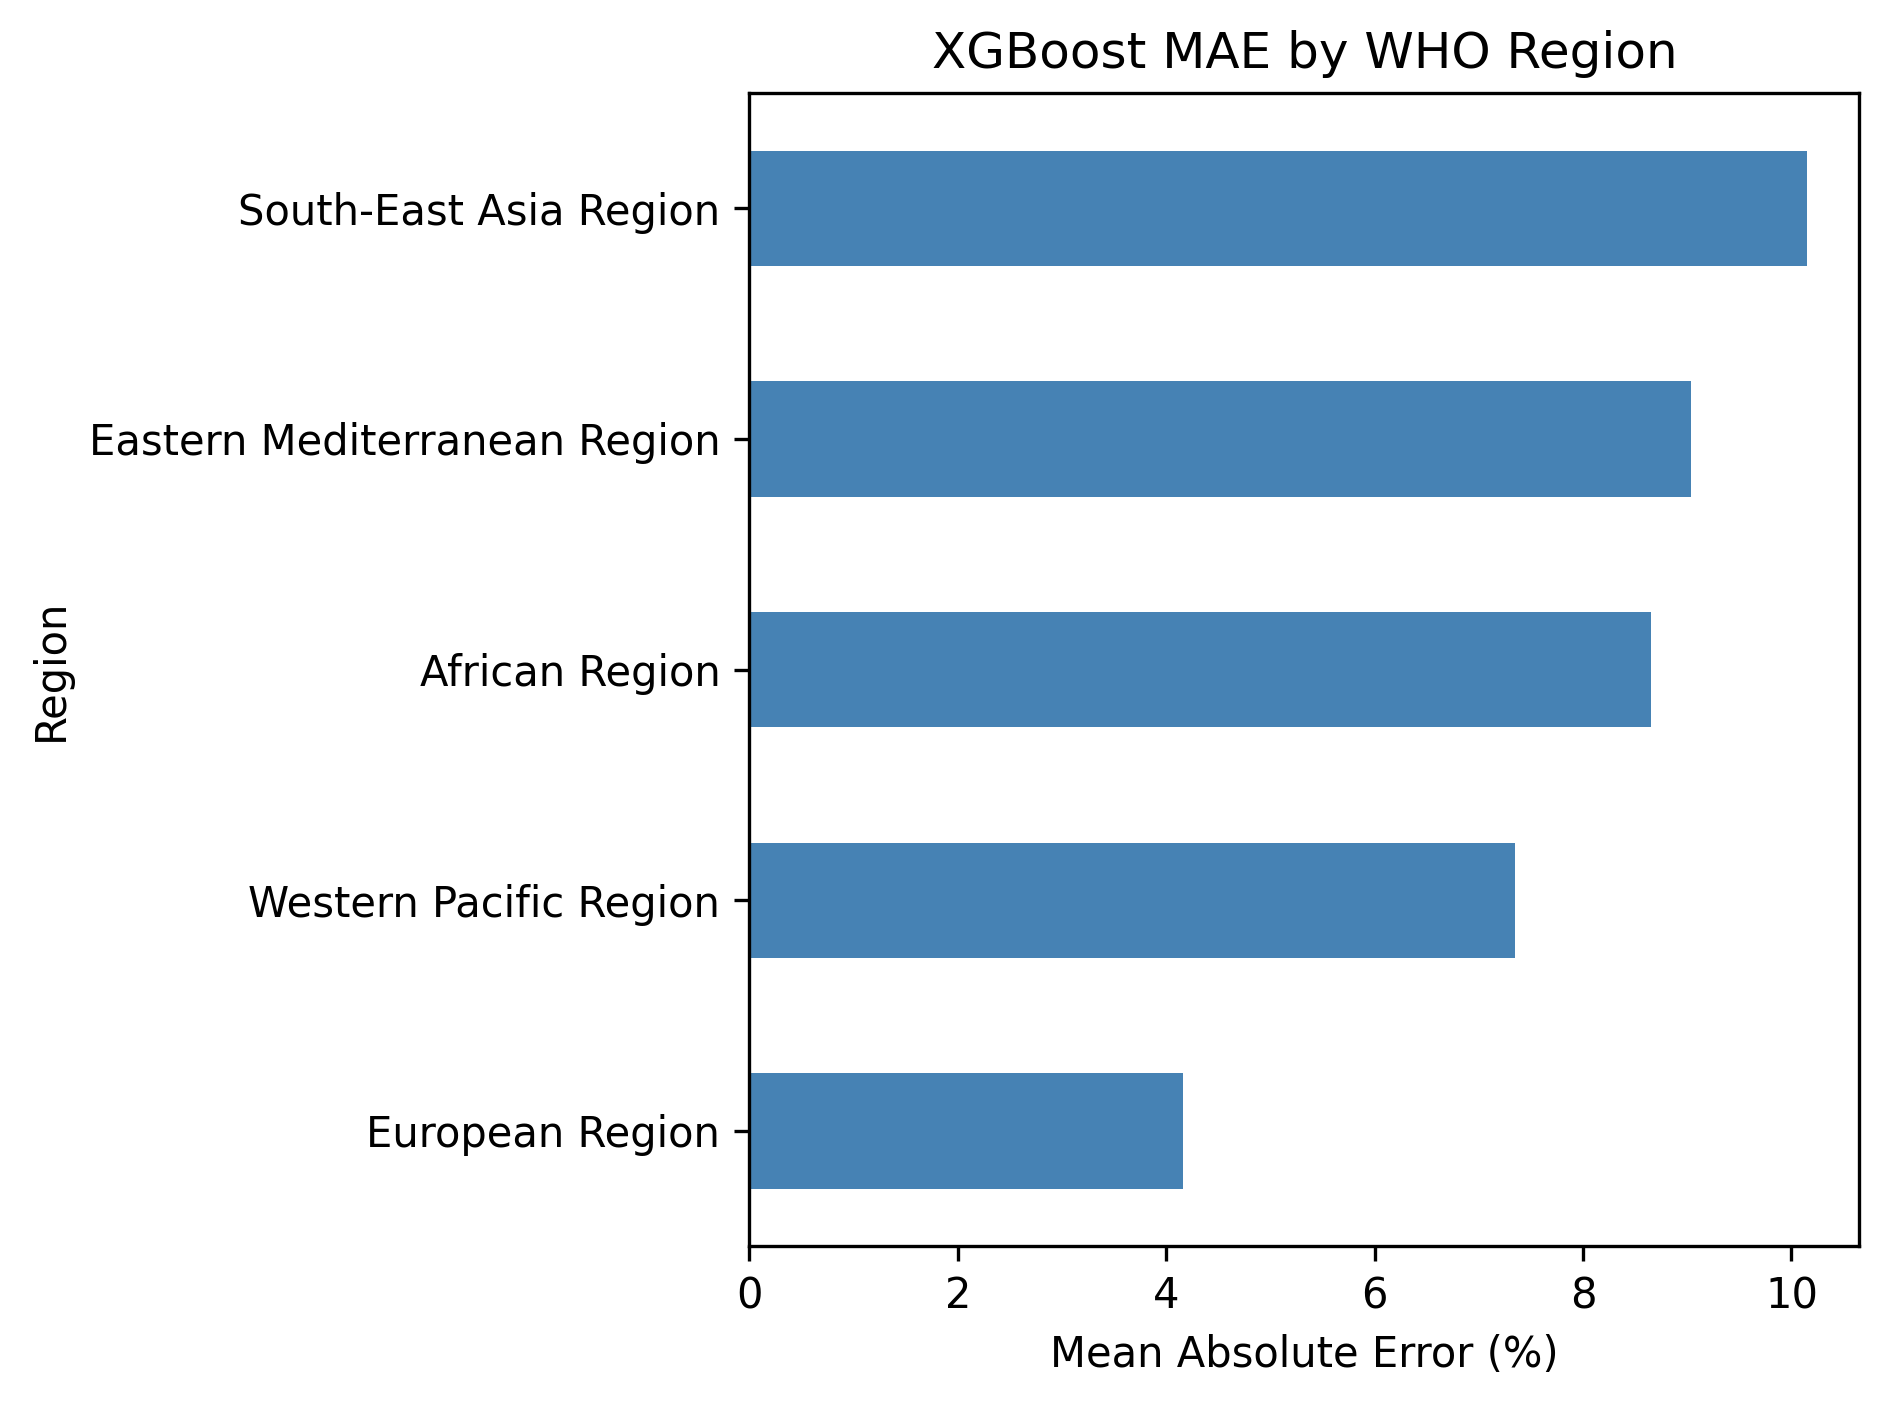
\includegraphics[width=0.85\textwidth]{mae_by_region.png}
\caption{XGBoost test MAE disaggregated by WHO region. The European Region achieves the lowest error (4.16\%), while South-East Asia shows the highest (10.14\%), reflecting disparities in GLASS data coverage.}
\label{fig:regional}
\end{figure}

Forecast accuracy varied substantially across regions. The European Region achieved the lowest MAE (4.16\%), reflecting comprehensive GLASS participation and high data consistency. The South-East Asia Region showed the highest MAE (10.14\%), approximately 2.4 times higher than Europe. This regional gradient closely mirrors the global AMR burden distribution documented by \citet{murray2022}, in which high-burden regions also tend to have weaker surveillance infrastructure.

\subsection{RAG Policy Q\&A System}

\begin{figure}[H]
\centering
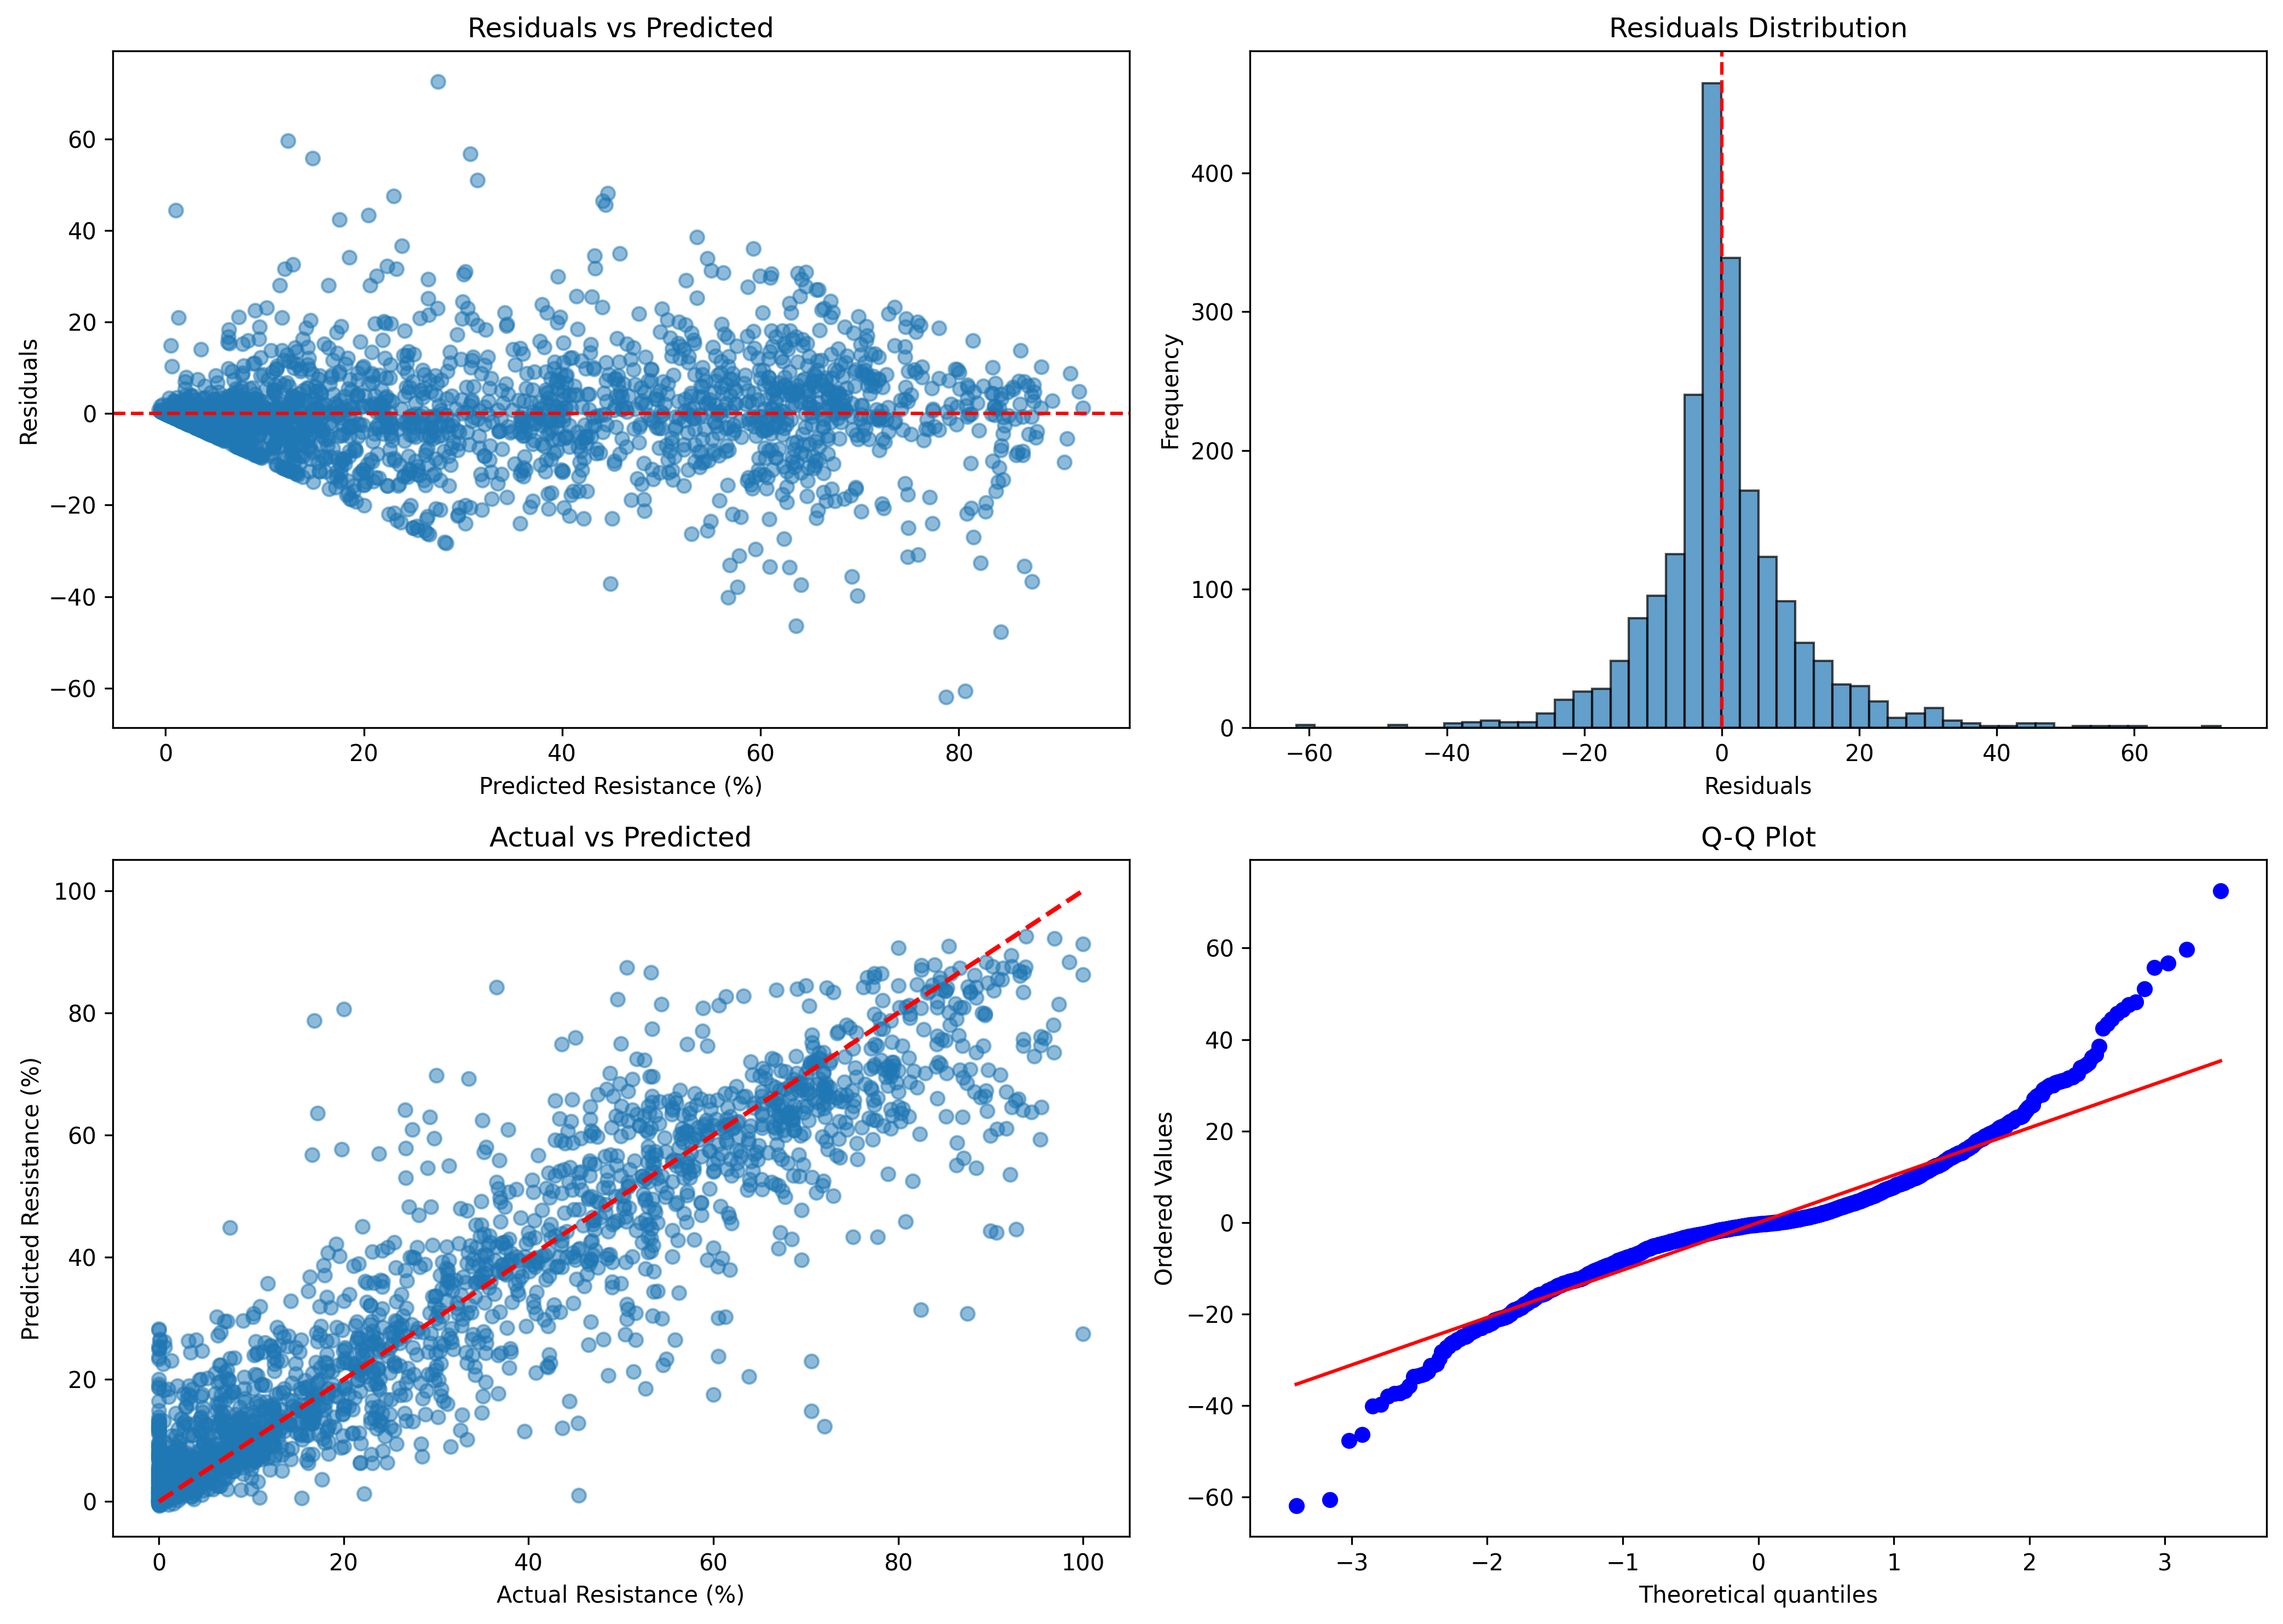
\includegraphics[width=0.85\textwidth]{error_analysis.png}
\caption{XGBoost residual and error analysis on the 2023 test set. Most predictions fall within a narrow error range, with larger errors concentrated in high-resistance observations.}
\label{fig:error}
\end{figure}

We evaluated the RAG system on five predefined policy questions spanning antibiotic prioritization by region, treatment guidelines for resistant pathogens, regional forecast uncertainty, income-stratified resistance trends, and surveillance investment priorities. All five responses demonstrated: (1) accurate retrieval of relevant WHO policy excerpts, (2) correct attribution of retrieved sources without fabricated references, and (3) coherent integration of forecast findings into policy recommendations.

\textbf{Representative example.} Question: \textit{Which antibiotics should Southeast Asia prioritize preserving based on resistance forecasts?} The system correctly identified carbapenem-resistant ESKAPE pathogens as critical threats, recommended prioritizing Access-group antibiotics per the AWaRe classification, connected the region's high forecast uncertainty (MAE: 10.1\%) to surveillance infrastructure gaps, and recommended targeted investment in antibiotic stewardship and laboratory capacity consistent with WHO LMIC guidance.

% ---------- 5. Discussion ----------
\section{Discussion}

\subsection{Forecasting Performance}

Our results confirm XGBoost as an effective model for short-term AMR resistance rate forecasting from WHO surveillance data (MAE: 7.07\%, R\textsuperscript{2}: 0.854). The dominance of the resistance lag feature (50.5\%) indicates that near-term AMR forecasting is primarily autoregressive: past resistance strongly predicts future resistance. This has practical implications for resource-constrained settings, as lag-only features capture the majority of the predictable signal.

The near-equivalent performance of gradient boosting and LSTM models (MAE spread $< 0.15$ percentage points) suggests that the three-year temporal window does not provide sufficient depth for LSTM to exploit its sequential modeling advantage. Extended GLASS time series may reveal more meaningful gains from deep learning, consistent with findings from longer epidemic datasets \citep{chimmula2020}.

The regional MAE gradient reflects inequities in GLASS participation. Expanding GLASS enrollment in high-burden regions would simultaneously improve AMR surveillance and forecasting accuracy.

\subsection{RAG System Evaluation}

The RAG pipeline produced grounded, policy-relevant answers by combining retrieved WHO document excerpts with XGBoost forecast context. The prompt-level citation constraint effectively prevented hallucinated references, a known failure mode of large language models \citep{lewis2020}. Expanding the knowledge base with complete WHO GLASS annual reports and national AMR action plans would substantially improve retrieval coverage.

\subsection{Limitations}

Several limitations should be acknowledged. First, the dataset spans only three years (2021--2023), restricting the model's ability to capture multi-year emergence trajectories. Second, GLASS data represents a geographically non-random sample weighted toward countries with existing surveillance capacity, introducing selection bias in regional comparisons. Third, the RAG knowledge base is small and manually curated. Fourth, Phi-3 Mini has lower reasoning capacity than larger frontier models for complex multi-step queries.

\subsection{Future Directions}

Future work should explore: (1) integration of 2024 GLASS data to extend the temporal window; (2) inclusion of complete WHO policy documents in the RAG knowledge base; (3) evaluation of the Temporal Fusion Transformer for longer-range forecasting; (4) domain-adapted sentence embeddings trained on AMR literature; and (5) formal automated evaluation of RAG response faithfulness using frameworks such as RAGAS.

% ---------- 6. Conclusion ----------
\section{Conclusion}

This paper presented an integrated framework for AMR resistance rate forecasting and evidence-grounded policy question answering using WHO GLASS surveillance data. Across six benchmarked models, XGBoost \citep{chen2016} achieved the best forecasting performance (MAE: 7.07\%, R\textsuperscript{2}: 0.854), representing an 83.1\% improvement over the naive baseline. The prior-year resistance lag accounted for over half of model predictive power, and regional forecast accuracy tracked closely with GLASS data quality.

We additionally implemented a RAG pipeline \citep{lewis2020} producing grounded, source-attributed responses to AMR policy questions without fabricated citations, demonstrating the feasibility of integrating ML-based surveillance forecasts into a locally deployable policy decision support tool.

As AMR is projected to cause 10 million deaths per year by 2050 \citep{oneill2016, dekraker2016}, tools that translate global surveillance data into actionable policy insights are urgently needed. Expanding GLASS participation and coupling those data streams with forecasting and retrieval systems represents a concrete step toward evidence-based AMR governance at global scale.

% ---------- References ----------
\bibliographystyle{plainnat}
\bibliography{references}

\end{document}
